\chapter{生物}
在本章中,我将介绍无机环境与异世界生物之间的关系。生物从无机环境中诞生,生物活动时刻改变着无机环境,而变化的无机环境又反作用于生物本身。如此循环往复,最终达到平衡。

本章涉及了一些生物学,尤其是生态学的内容,这可以帮助我们更完美地描绘异世界的“外貌”。

\section{生物的演化}

\section{生态系统}
\textbf{生态系统}(ecosystem)是指在一个特定环境内,由生物群落与非生物因素相互作用而形成、能够自我维持的整体。

生态系统的范围没有固定的大小。小到一个池塘,大到沙漠、草原。一个星球上最大的生态系统叫\textbf{生物圈}(biosphere),包含了其上所有生态系统,是全部生物及其环境的总和。

\subsection{种群和群落}
在生态学上,\textbf{种群}(population)是指在一定空间范围内同时生活的同种生物的全部个体。在同一时间内,聚集在一定区域内各种生物种群的集合则称为\textbf{群落}(community)。

\subsection{食物网}

\section{演替}
\textbf{演替}(ecological succession)是一个群落的物种结构随时间变化的过程,是由低级到高级、由简单到复杂、一个阶段接着一个阶段、一个群落代替另一个群落的自然演变现象。演替可分为初生演替和次生演替两大类。

\subsection{初生演替}
如果一个地区从未被生物定居过(或者彻底清除了一切生物),生物从无开始的演替,称为\textbf{初生演替}(primary succession)。这是一个“巨岩变细石,石上长青苔”的过程,会经历极其漫长的岁月。

\begin{figure}[htbp]
    \centering
    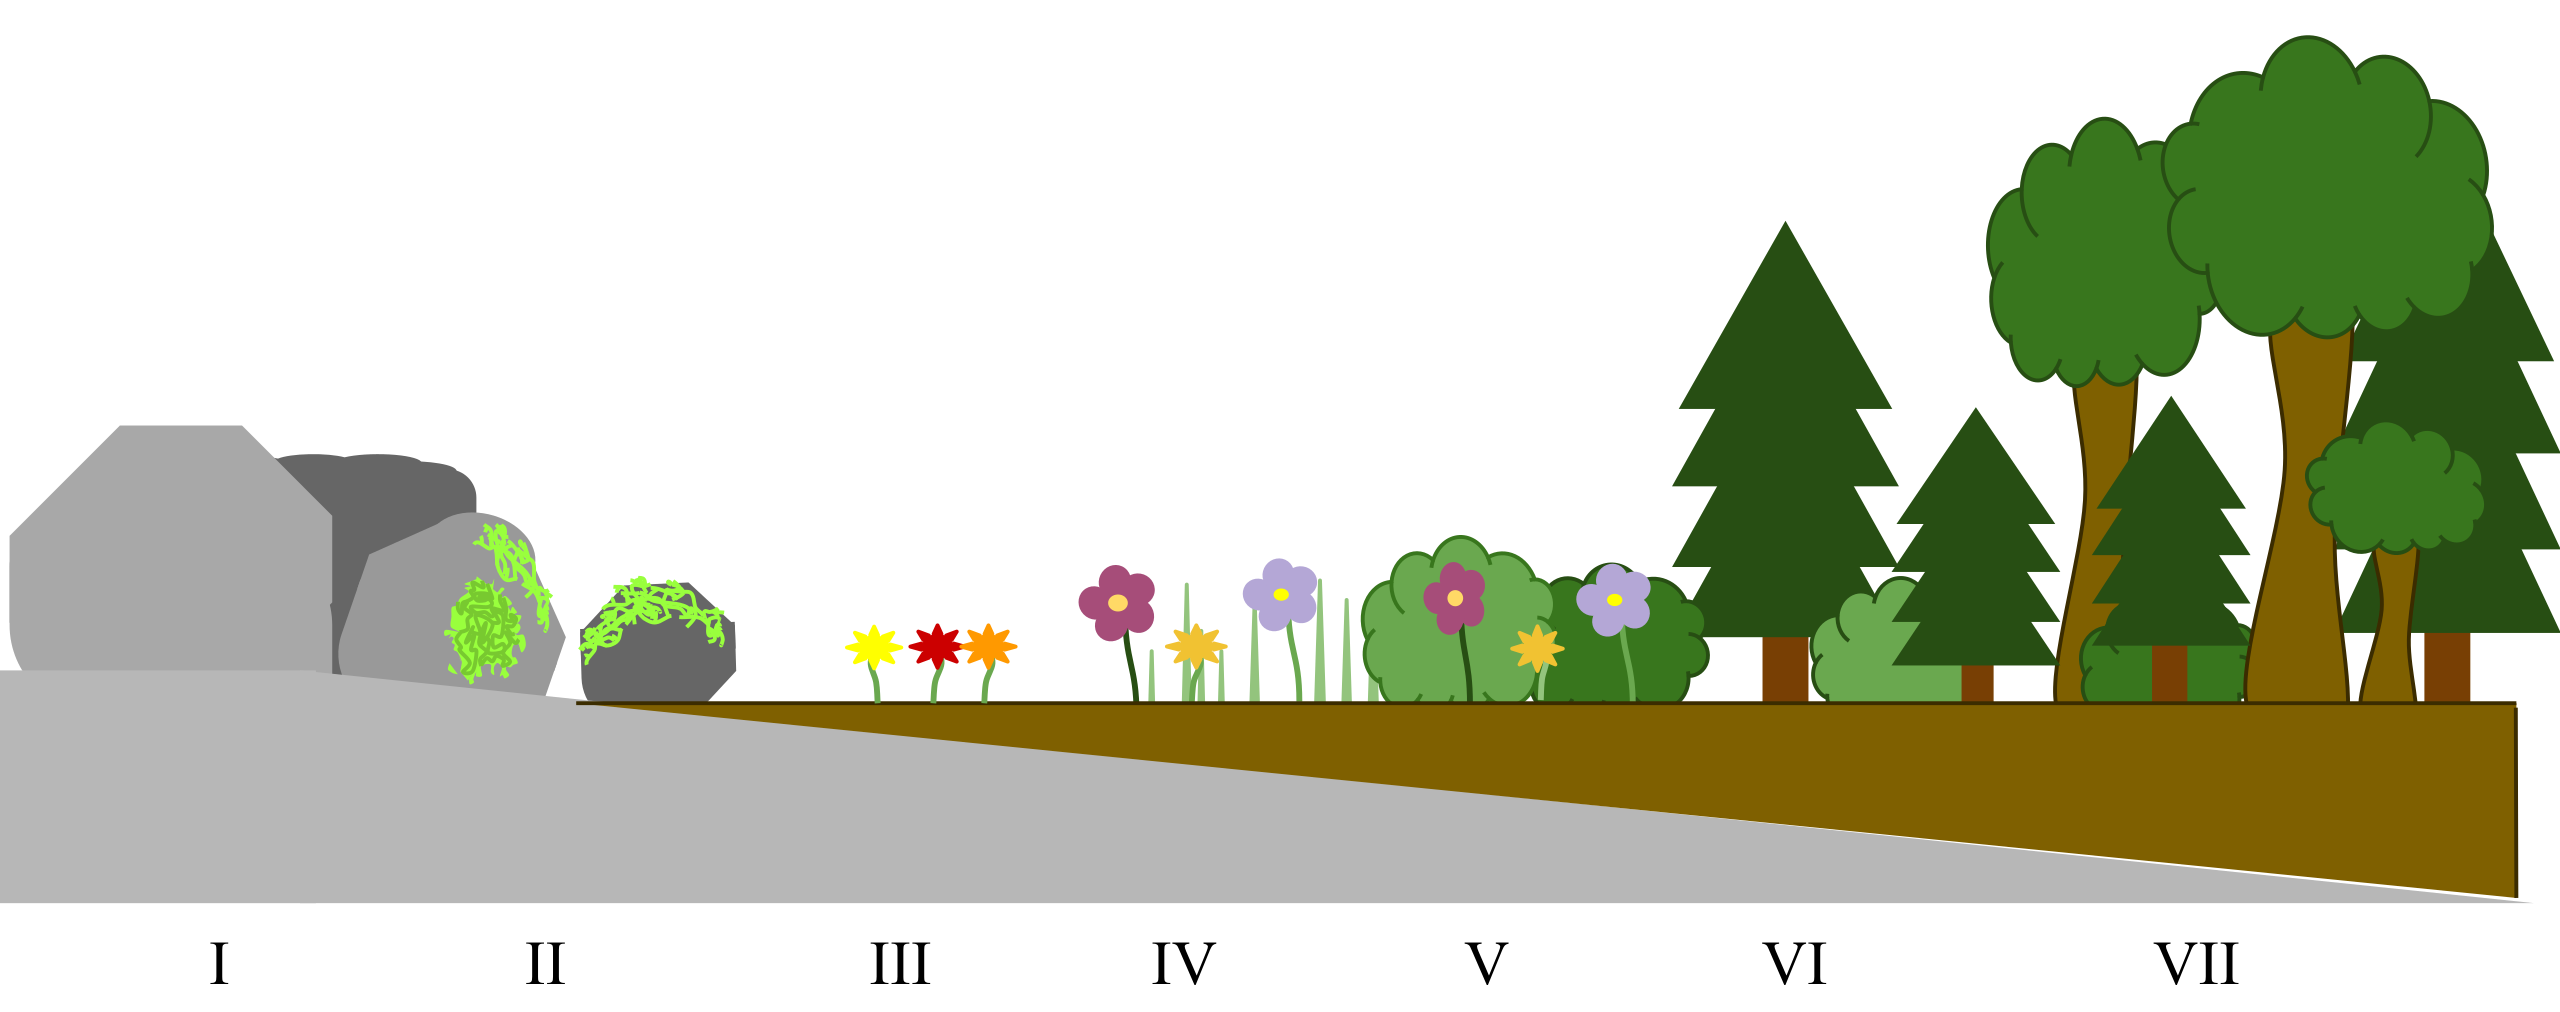
\includegraphics[width=400pt]{images/primary-succession.png}
    \caption{初生演替的各个阶段}
    \label{fig:primary-succession}
\end{figure}

如图 \ref{fig:primary-succession} 展示了初生演替的7个阶段。

遥想亿万斯年以前,陆地上全是一望无际的、光秃秃的岩石。这一时期(阶段I)岩石上没有定居任何生命,称为裸岩阶段。

\subsection{次生演替}
与初生演替不同,\textbf{次生演替}(secondary succession)始于一场突发事件(如野火、飓风),致使原有生态系统中种群数量极度减少,但土壤并未受到十分严重的破坏的环境中。而初生演替的群落则缺乏土壤。

\begin{figure}[htbp]
    \centering
    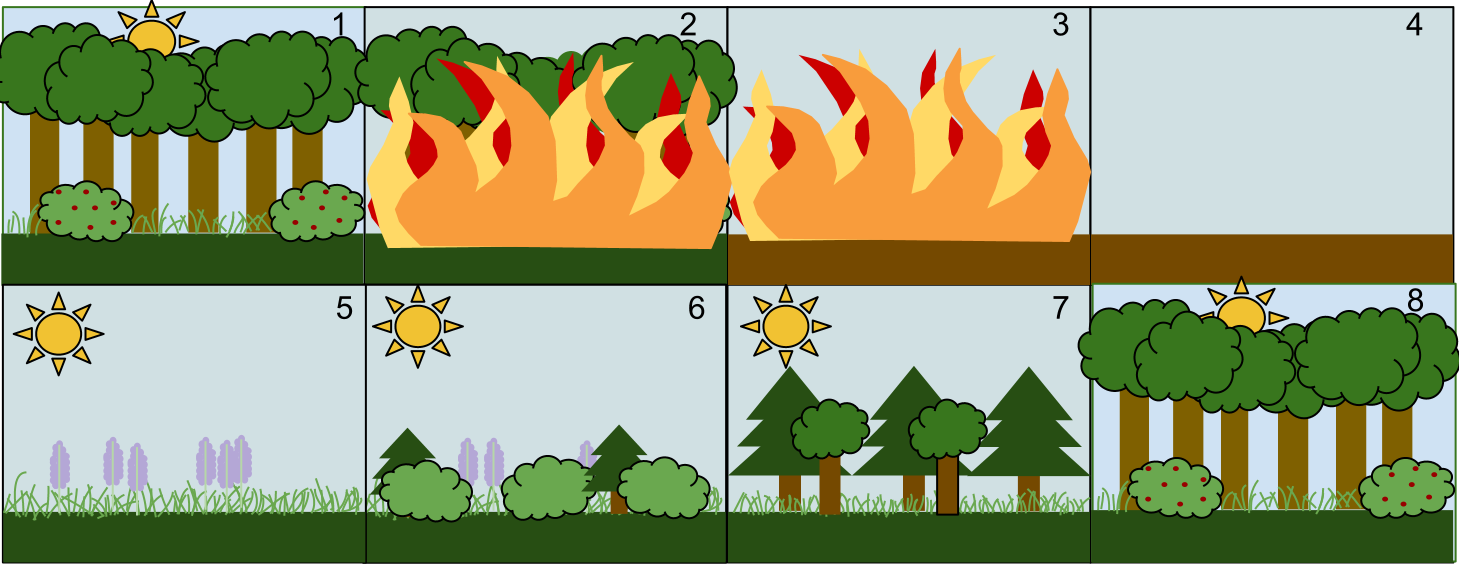
\includegraphics[width=400pt]{images/secondary-succession.png}
    \caption{次生演替的各个阶段}
    \label{fig:secondary-succession}
\end{figure}
